\documentclass[presentation,9pt]{beamer}
%\documentclass[handout,9pt]{beamer}

\mode<presentation>
{
%  \usetheme{Warsaw}
  % or ...
\usetheme{Goettingen}
%\usetheme{Hannover}

%\usecolortheme{crane}
%\usecolortheme{beaver}
%\usecolortheme{beetle}
%\usecolortheme{dolphin}
%\usecolortheme{whale}
%\usecolortheme{wolverine}
%\usecolortheme{albatross}
%  \setbeamercovered{transparent}
  % or whatever (possibly just delete it)
}


\setbeamertemplate{navigation symbols}{}

\usepackage[utf8]{inputenc}
\usepackage[spanish, es-tabla, es-nodecimaldot]{babel}

\usepackage{listings}
\usepackage{tikzsymbols}

%\usepackage{times}
%\usepackage[T1]{fontenc}
% Or whatever. Note that the encoding and the font should match. If T1
% does not look nice, try deleting the line with the fontenc.


\title[RNP series temp.] % (optional, use only with long paper titles)
{RNPs aplicadas a reconocimiento de patrones en registros electromiográficos de insectos.}

%\subtitle

\author[HS, SP]
{Héctor Salas (\small hecsalms@gmail.com)\\ 
G. Sebastián Pedersen (\small sebasped@gmail.com)}%\inst{1}}
% - Give the names in the same order as the appear in the paper.
% - Use the \inst{?} command only if the authors have different
%   affiliation.

%\institute[] % (optional, but mostly needed)
%{3er. Ciclo de Charlas de Matemática --- ICI --- UNGS 
%  \inst{1}%
%  Instituto de Industria\\
%  Universidad Nacional de General Sarmiento
%  \and
%  \inst{2}%
%  Department of Theoretical Philosophy\\
%  University of Elsewhere}
% - Use the \inst command only if there are several affiliations.
% - Keep it simple, no one is interested in your street address.
%}

\date[] % (optional, should be abbreviation of conference name)
{Mar 03 de Diciembre de 2019\\ 
%\vspace{.5cm}
%{
%\small\url{subir_la_charla_a_github_y_poner_la_url}
}



% If you have a file called "university-logo-filename.xxx", where xxx
% is a graphic format that can be processed by latex or pdflatex,
% resp., then you can add a logo as follows:

% \pgfdeclareimage[height=0.5cm]{university-logo}{university-logo-filename}
% \logo{\pgfuseimage{university-logo}}


% Delete this, if you do not want the table of contents to pop up at
% the beginning of each subsection:
%\AtBeginSubsection[]
%{
%  \begin{frame}<beamer>{Outline}
%    \tableofcontents[currentsection,currentsubsection]
%  \end{frame}
%}


% If you wish to uncover everything in a step-wise fashion, uncomment
% the following command: 

%\beamerdefaultoverlayspecification{<+->}




\begin{document}

\begin{frame}
  \titlepage
  \vspace{-.5cm}
  \begin{abstract}
  	{Se aplican redes neuronales profundas para un problema de clasificación de series temporales provenientes de mediciones electromiográficas  de vinchucas.}
  \end{abstract}
  
\end{frame}




\section{El problema}

%\subsection{Expresiones}
\begin{frame}{Una serie temporal típica}
	Corresponde al insecto en reposo, insertando el pico, comiendo.

	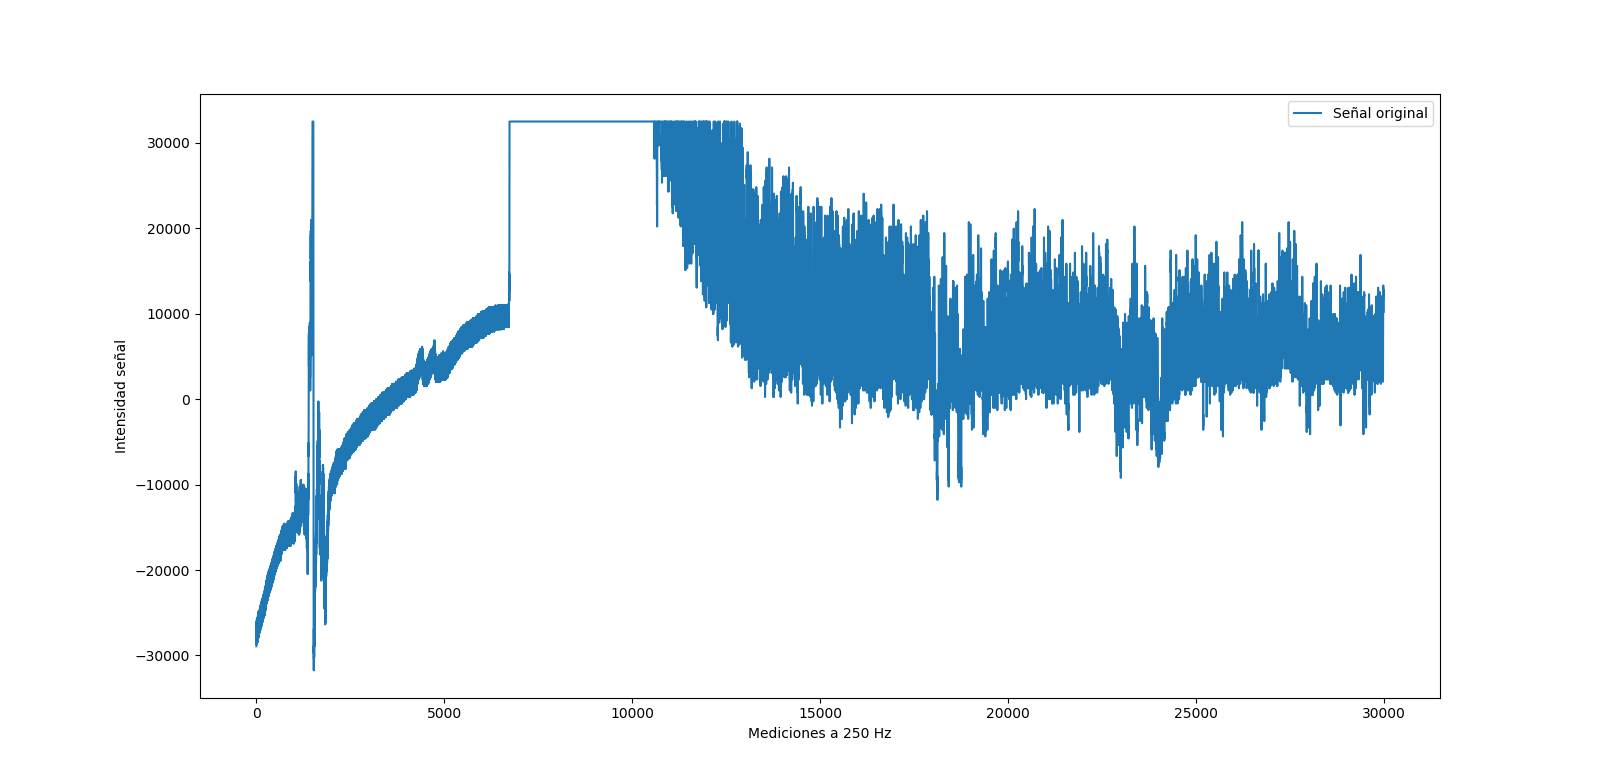
\includegraphics[width=.8\textwidth]{./senialOrig.png}
	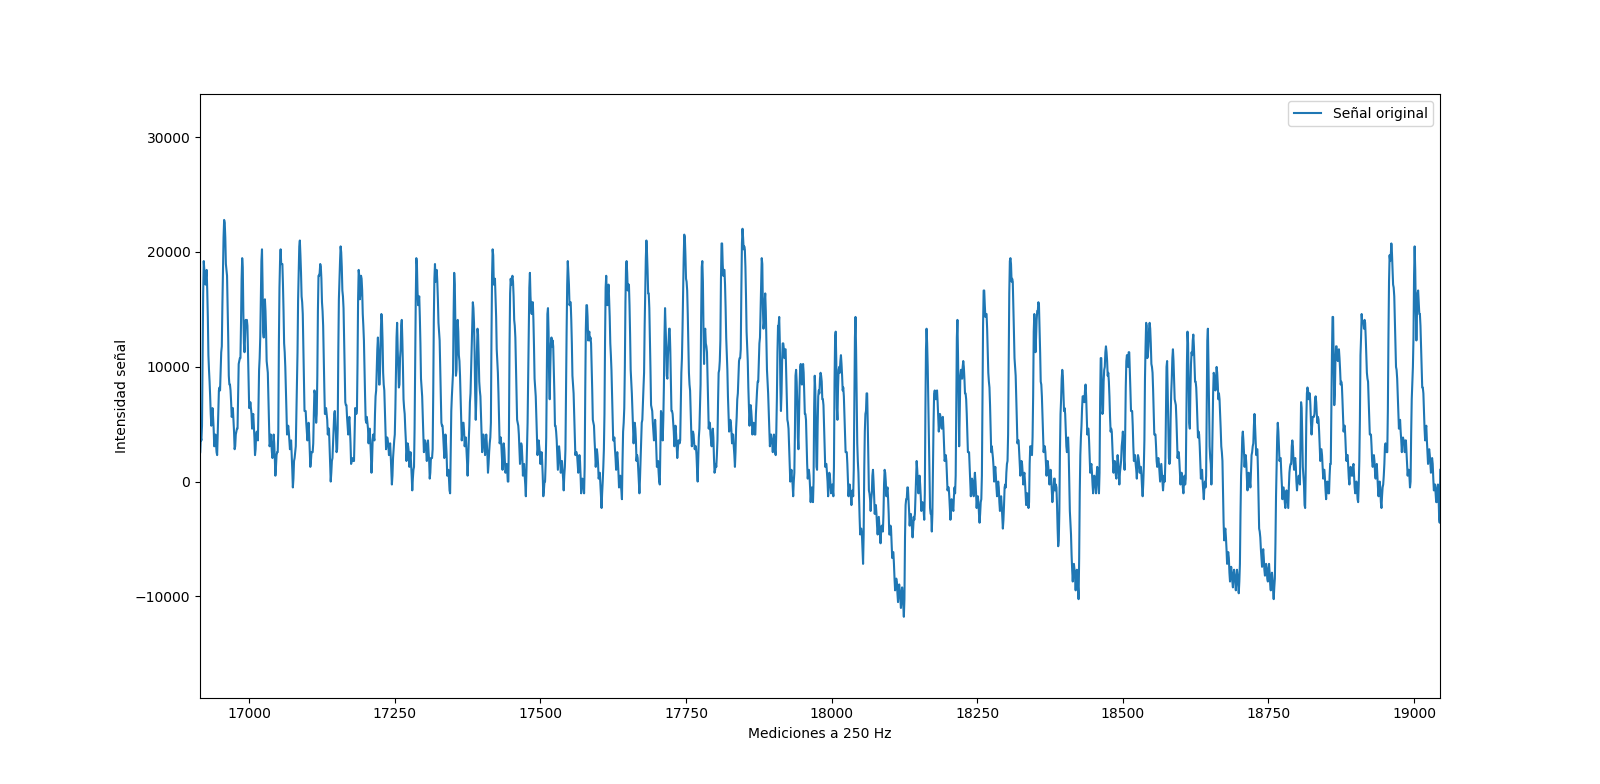
\includegraphics[width=.8\textwidth]{./senial2Orig.png}

\end{frame}



\begin{frame}{Preproceso de las series por BEADS\footnote{\url{http://www.laurent-duval.eu/siva-beads-baseline-background-removal-filtering-sparsity.html}}}
	
	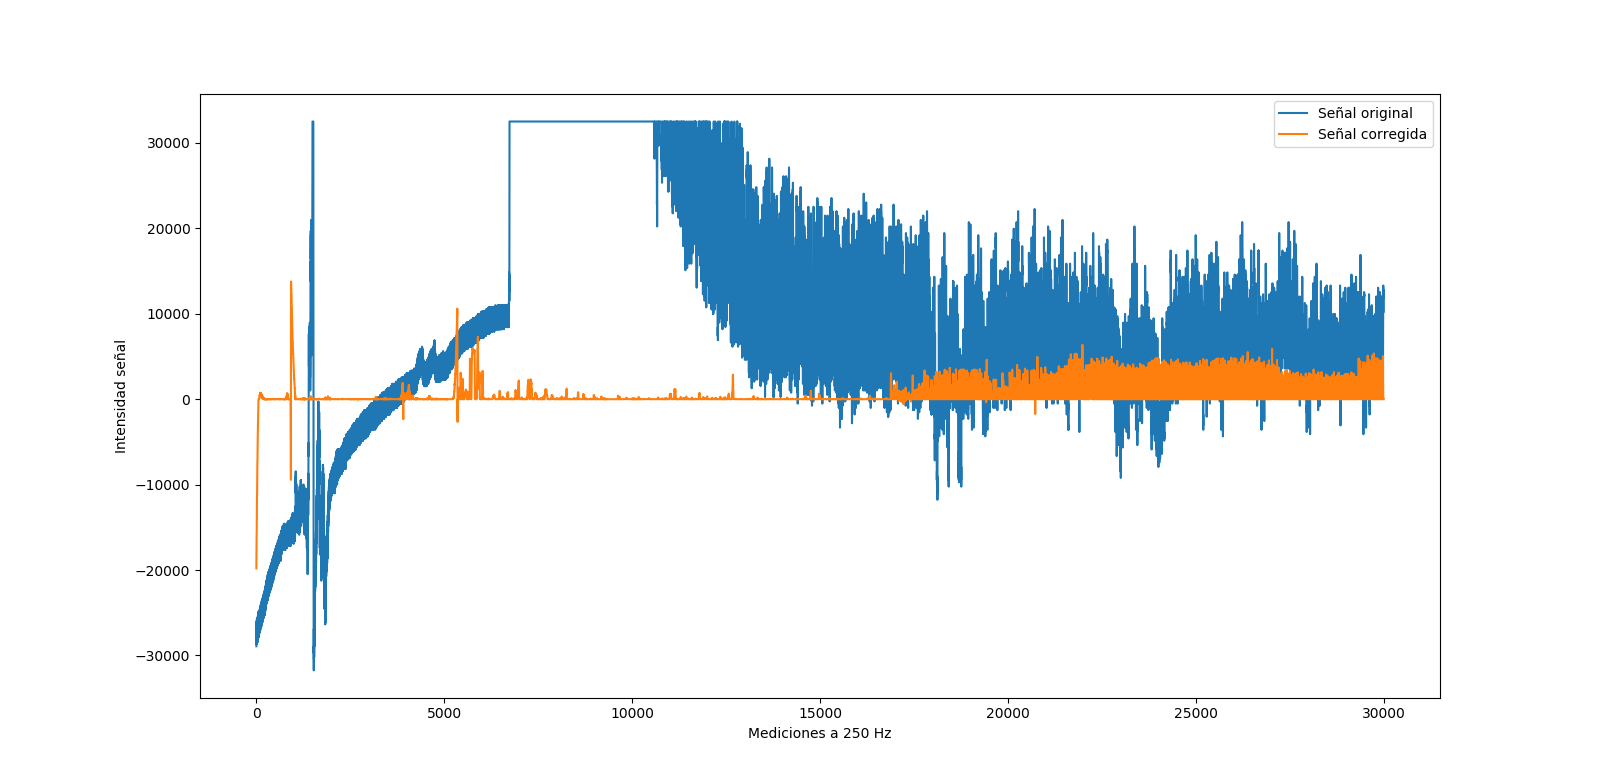
\includegraphics[width=.8\textwidth]{./senial.png}
	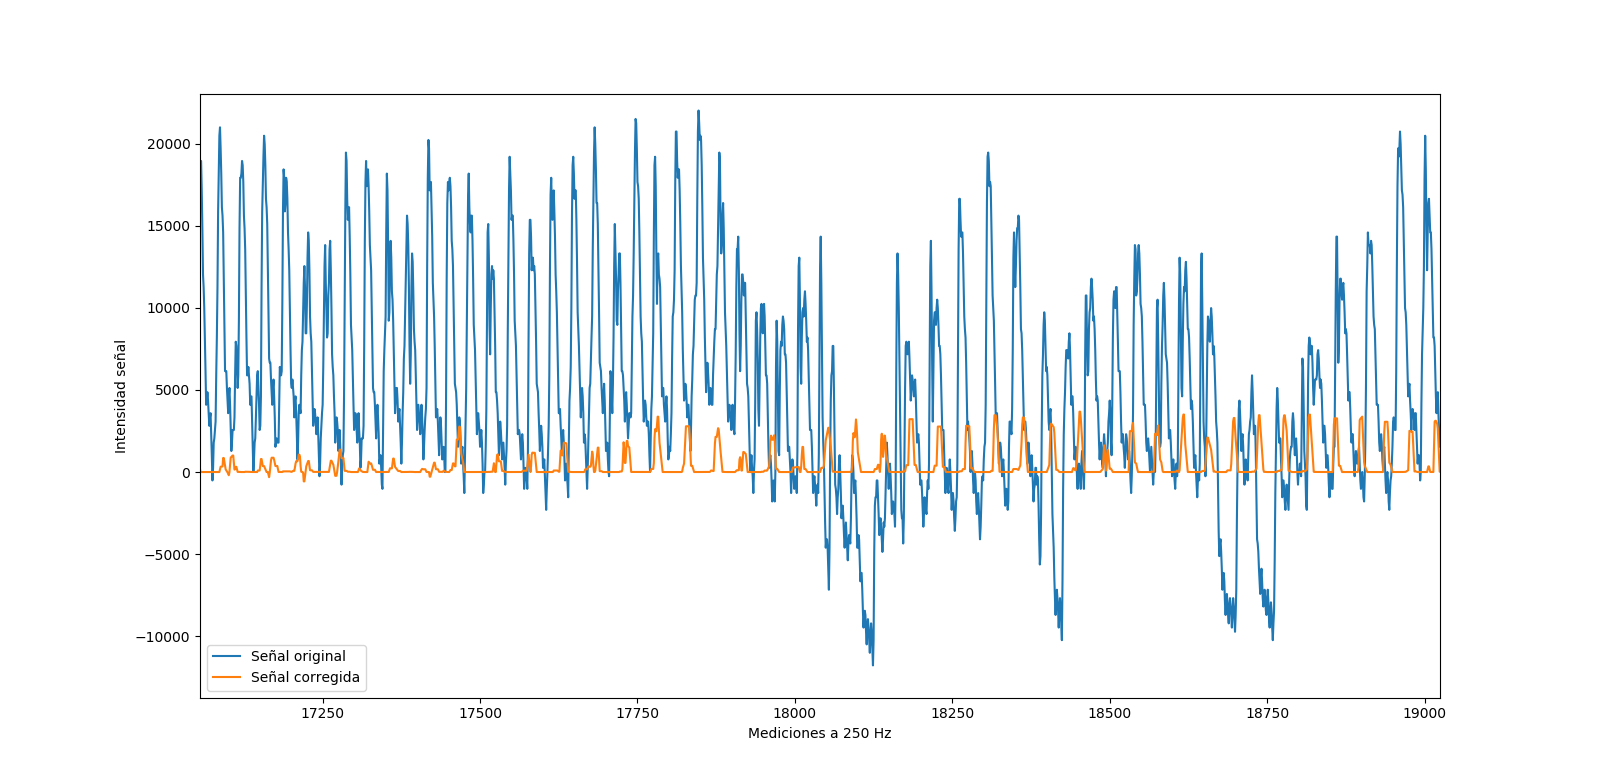
\includegraphics[width=.8\textwidth]{./senial2.png}

\end{frame}

\begin{frame}{El problema de clasificación}
	Automatizar el proceso de detección inicio/fin de región de interés (con picos).
	
	Distinguir regiones sin pico de regiones con pico.
	
	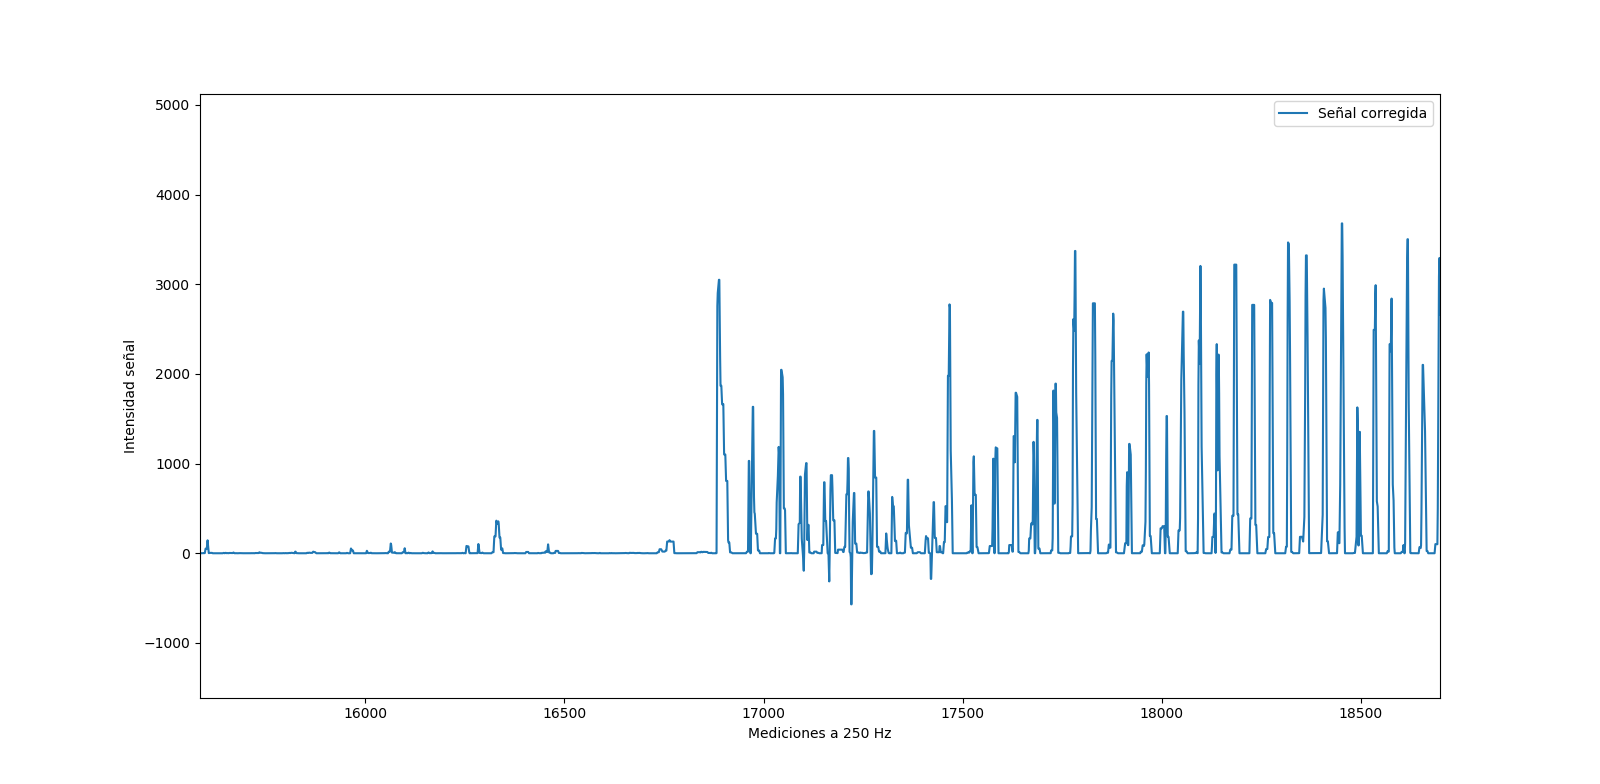
\includegraphics[width=\textwidth]{./zonaSinConPico.png}
	
	Sin pico: el insecto no está comiendo.

	Con pico: el insecto está comiendo (región de interés).

\end{frame}



\begin{frame}{Partición en ventanas para clasificar}
	Se parte la serie en ventanas, cada una clasificada Sí/No región de interés.
	
%	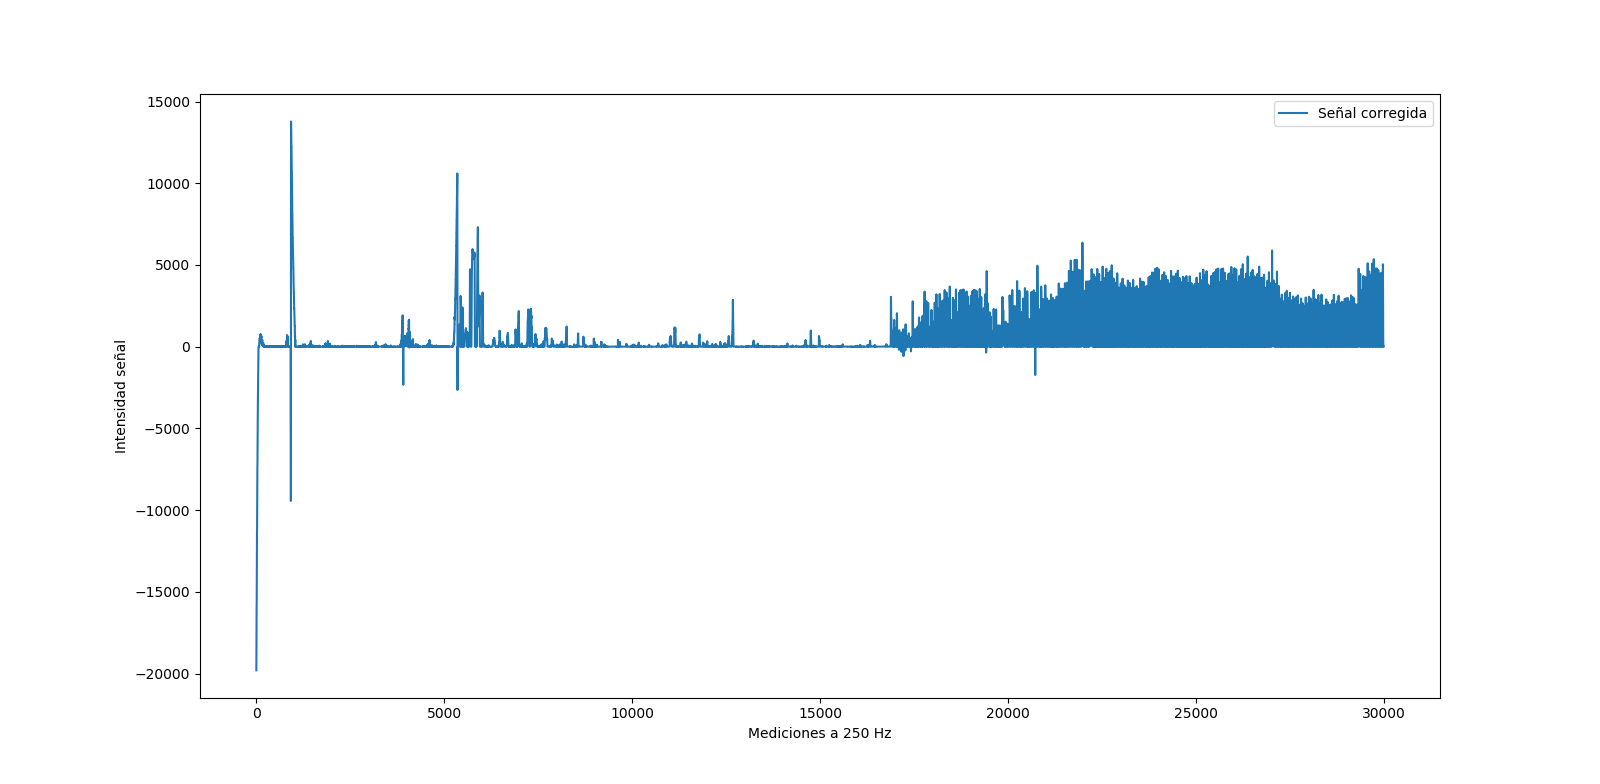
\includegraphics[width=\textwidth]{./separacionVentanas.png}
	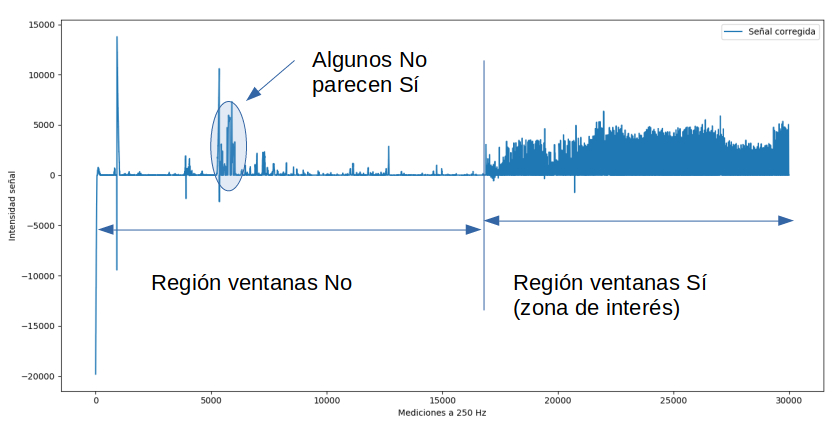
\includegraphics[width=\textwidth]{./separacionVentanasBien.png}

	Luego a la primera Sí: inicio región de interés

	A la primera No: fin región de interés
	
\end{frame}




\section{Las RNPs probadas}
\begin{frame}{Primeras redes}
	Redes convolucionales con estas arquitecturas:
	\begin{itemize}
		\item Input: ventanas de 6 seg. O sea seriel temporal 1D de 1500 datos (250 Hz).
		\item Convolucional 1D de 5x60 (stride=1 o 2, padding=20)
		\item ReLu
		\item Convolucional 1D de 10x30 (stride=1, padding=10)
		\item Max Pooling de 4 o de 2
		\item ReLu 
		\item FC de 1830 a 300 (luego tanh)
		\item Prueba agregando FC a 300/400
		\item FC de 300 a Sí/No
	\end{itemize}
	
	Accuracy de aprox. 90-92\%.
	
	
%	\begin{block}{}
%		Herramienta más popular: PLT (Production Logging Tool)
%	\end{block} 
\end{frame}




\begin{frame}{Segundas redes: algo más profundas}
	Una red convolucional con esta arquitectura:
	\begin{itemize}
		\item Input: ventanas de 6 seg. O sea seriel temporal 1D de 1500 datos (250 Hz).
		\item Convolucional 1D de 5x60 (stride=1, padding=30)
		\item ReLu
		\item Convolucional 1D de 10x30 (stride=2, padding=20)
		\item Max Pooling de 2
		\item ReLu 
		\item Convolucional 1D de 20x15 (stride=2, padding=30)
		\item Max Pooling de 2
		\item ReLu
		\item FC de 580 a 300 (luego tanh)
		\item FC de 300 a 100 (luego tanh)
		\item FC de 100 a Sí/No
	\end{itemize}

	\begin{columns}
		\column{0.2\textwidth}
	Accuracy de aprox. 93-94\%.
		
		\column{0.8\textwidth}
			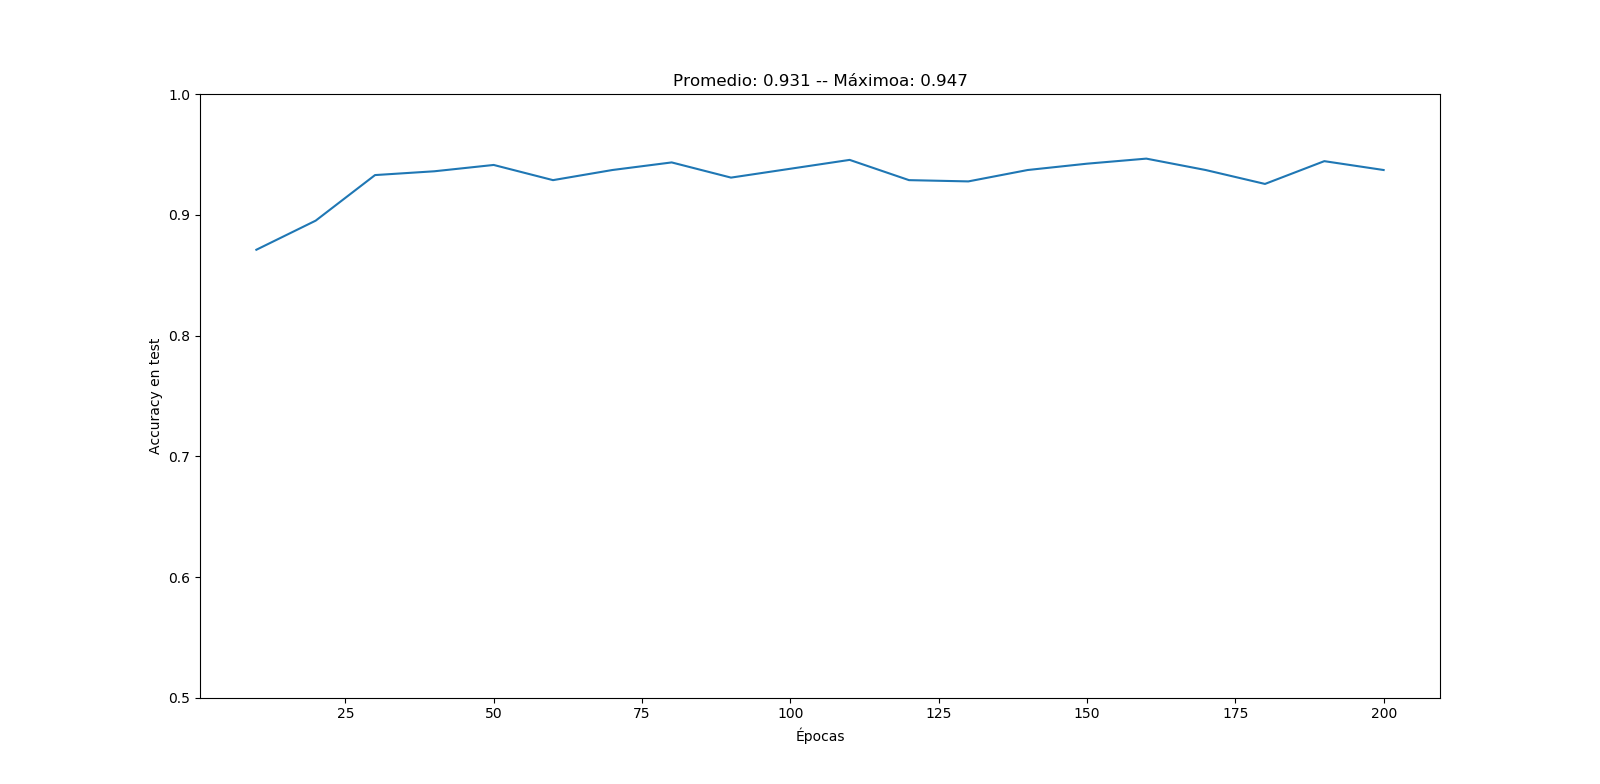
\includegraphics[width=.9\textwidth]{./cnn_v7_ball.png}
		
	\end{columns}	

\end{frame}




\begin{frame}{Terceras redes: con ventanas de 1 seg.}
	Una red convolucional con esta arquitectura:
	\begin{itemize}
		\item Input: ventanas de 1 seg. O sea seriel temporal 1D de 250 datos (250 Hz).
		\item Convolucional 1D de 5x60 (stride=1, padding=30)
		\item ReLu
		\item Convolucional 1D de 10x30 (stride=2, padding=30)
		\item Max Pooling de 2
		\item ReLu 
		\item Convolucional 1D de 20x15 (stride=2, padding=30)
		\item Max Pooling de 2
		\item ReLu
		\item FC de 580 a 300 (luego tanh)
		\item FC de 300 a 100 (luego tanh)
		\item FC de 100 a Sí/No
	\end{itemize}
	
		\begin{columns}
		\column{0.2\textwidth}
		Accuracy de aprox. 94\%.
		
		\column{0.8\textwidth}
		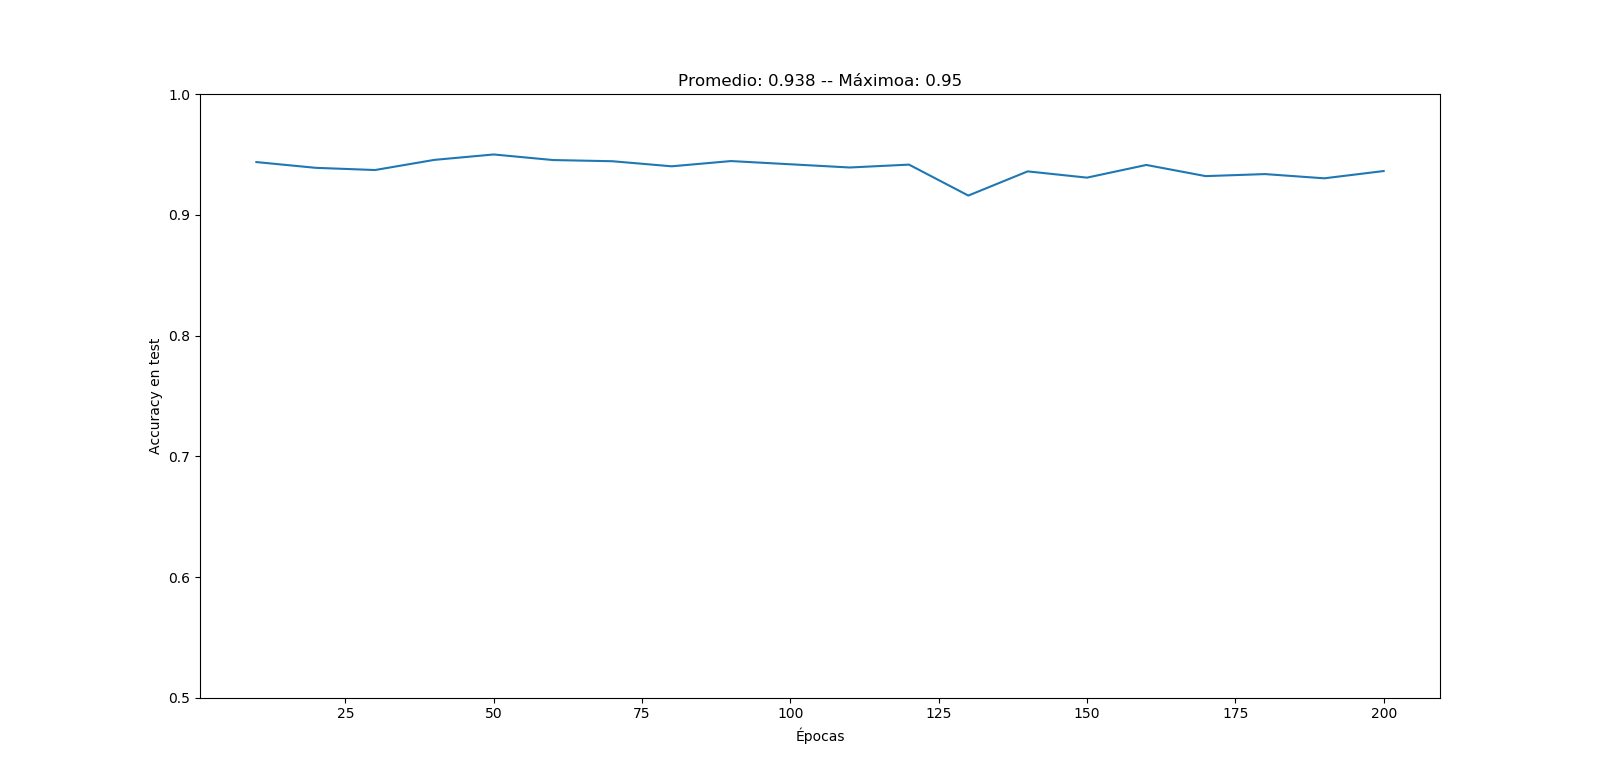
\includegraphics[width=.9\textwidth]{./cnn_v7_1seg_b1000.png}
		
	\end{columns}
	
\end{frame}



\begin{frame}{Terceras redes: con ventanas de 1 seg.}
Ídem antes, ahora normalizando los datos
%	\begin{itemize}
%		\item Input: ventanas de 1 seg. O sea seriel temporal 1D de 250 datos (250 Hz).
%		\item Convolucional 1D de 5x60 (stride=1, padding=30)
%		\item ReLu
%		\item Convolucional 1D de 10x30 (stride=2, padding=30)
%		\item Max Pooling de 2
%		\item ReLu 
%		\item Convolucional 1D de 20x15 (stride=2, padding=30)
%		\item Max Pooling de 2
%		\item ReLu
%		\item FC de 580 a 300 (luego tanh)
%		\item FC de 300 a 100 (luego tanh)
%		\item FC de 100 a Sí/No
%	\end{itemize}
	
	Accuracy de aprox. 95-96\%.
	
	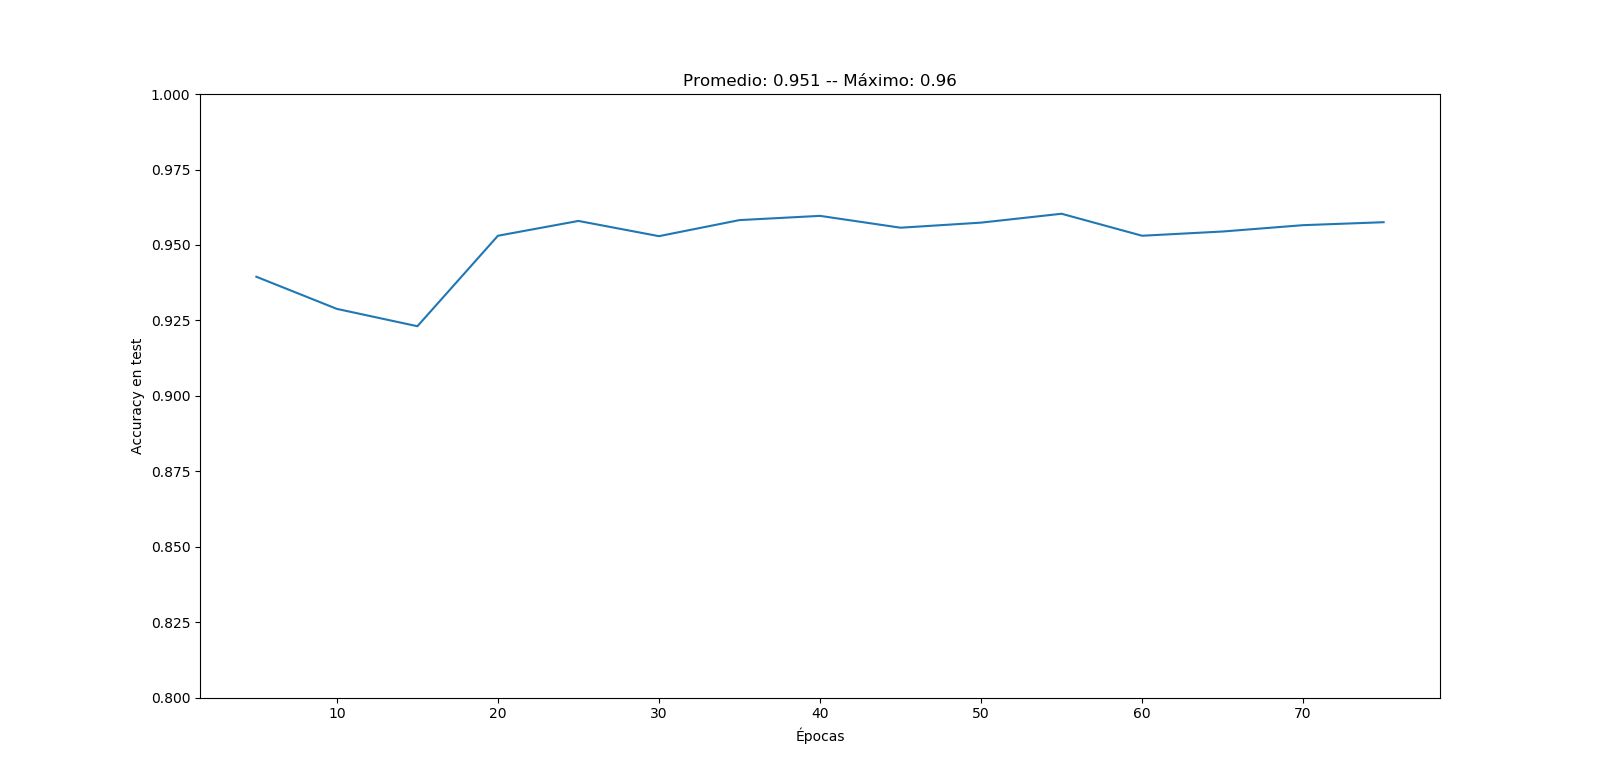
\includegraphics[width=\textwidth]{./cnn_v7_1seg_normalizado_b5000.png}
	
	\end{frame}


\begin{frame}{Cuarta red: con las FFTs de las ventanas de 1 seg.}
	Prueba rápida anoche:
		\begin{itemize}
			\item Input: FFTs de las ventanas de 1 seg.% O sea seriel temporal 1D de 250 datos (250 Hz).
			\item Convolucional 1D de 5x60 (stride=1, padding=30)
			\item ReLu
			\item Convolucional 1D de 10x30 (stride=2, padding=30)
			\item Max Pooling de 2
			\item ReLu 
			\item Convolucional 1D de 20x15 (stride=2, padding=30)
			\item Max Pooling de 2
			\item ReLu
			\item FC de 580 a 100 (luego tanh)
%			\item FC de 300 a 100 (luego tanh)
			\item FC de 100 a Sí/No
		\end{itemize}
	
	Accuracy de aprox. 91-92\%.
	
	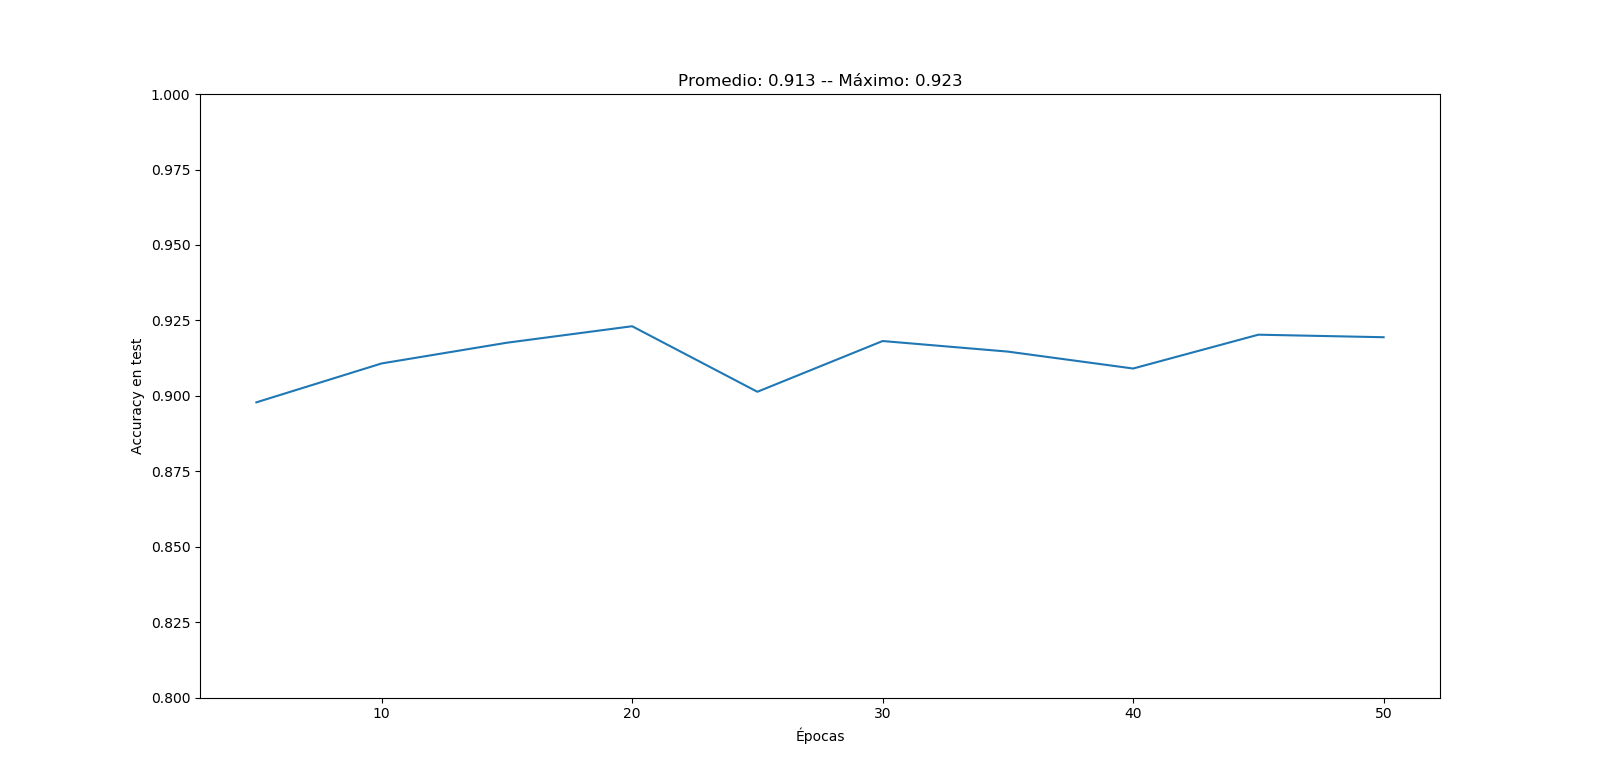
\includegraphics[width=.8\textwidth]{./cnn_v7_1seg_normalizado_fft_b1000.png}
	
	
\end{frame}




\section{Continuaciones futuras}

\begin{frame}{¿Cómo seguir a partir de aquí?}
	
	\begin{itemize}
		\item Probar con otras arquitecturas/parámetros para las CNNs.
		\item Probar otras Recurrentes.
		\item Input con series temporal + FFTs.
		\item Ensambles.
		\item Barrer el tamaño de la ventana más exhaustivamente.
		\item Barrer tamaño de batch más exhaustivamente.
		\item Reconocer más patrones en los registros.
	\end{itemize}
\end{frame}


	
	
\section{}
\begin{frame}
	\textbf{\centering\LARGE{¡GRACIAS!}}
\end{frame}


\end{document}


